\section{Background Research \& Analysis}

\subsection{Market Research \& Analysis}

\subsubsection{Coffee Research}
Coffee consumption in the United Kingdom has steadily increased over the past decade. In particular the past five years been seen an explosive increase, there are several theories as to why this is the case.

Firstly, instant coffee shops have become more common on our high streets. Companies such as Starbucks and Costa have been opening more stores as more Brits have been buying instant coffee, this doesn’t show any signs of slowing down either as Starbucks have recently announced 300 new stores to be opened over the next five years \cite{starbucks}.

Secondly, these brands have contributed to the newfound ‘coolness’ that is associated with coffee. 

Lastly, there is evidence that the economic climate has played a part in coffee’s rise. Also known as the ‘lipstick effect’, Britons have been unable to afford expensive treats for themselves so they have been spending on cheaper treats, a good example of which is coffee \cite{costa}.

This research is important to OptiCaff because it shows that the coffee industry is on the rise, it would not make business sense for us to invest in a declining industry.

\begin{center}
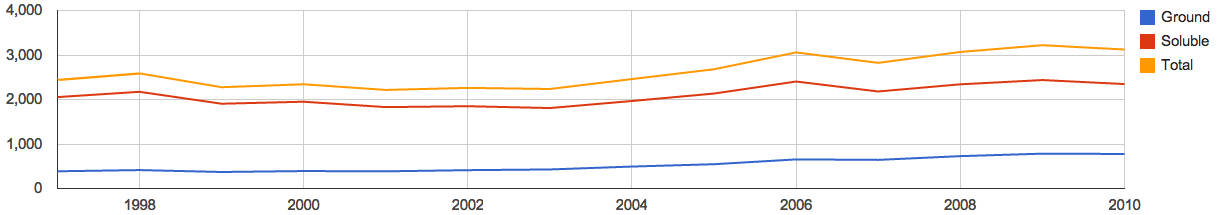
\includegraphics[trim = 0mm 0mm 0mm 0mm, clip, scale=0.4]{images/CaffeineGraph.png}
\end{center}

\subsubsection{Competitors Research \& Analysis}
\label{sec:competitors}
\subsection{Mobile Platform Research}
There are two mobile operating systems that OptiCaff could be deployed upon. The Android operating system created by Google requires applications to be written in Java which is a positive for the OptiCaff team, all members have Java development experience with one member having Android development experience. Using Android also means no special hardware is required to develop an application, the Android SDK is freely available and IDE’s are also free, Eclipse being an example of this \cite{Eclipse}. The app store for Android phones, Google Play, is a large marketplace that would give OptiCaff a great enough set of potential users.

``Google’s 10 Billion Android App Downloads: By the Numbers" \newline
A negative of Android is the result of it being open-source, manufacturers are able to create a separate version of Android just for their hardware, this means there are now lots of iterations of Android. Developing an application for all these different versions is difficult and OptiCaff would not be compatible with all phones at first.

iOS is the Apple iPhone’s operating system, it requires applications to be written in Objective C, no members in the OptiCaff team have any experience with Objective C. The only IDE available for developing iPhone applications is Xcode which is only available to OS X users, in other words, development is only possible on Apple computers, this is a requirement that is particularly limiting for a small development team. The Apple app store is currently the largest marketplace for mobile applications, although it is slightly ahead of Google Play. Finally, there is only one iteration of iOS, it is not licensed to other companies, the only complication is that there are a few versions running concurrently. This means that an app developed for the iPhone would likely work on all iPhones.

OptiCaff will be developed in Android, the reasons for this are that the members of the team are more comfortable with Java development and not all members of the team have an Apple computer and therefore would not be able to aid in development.

\subsection{Competitors Research \& Analysis}
\label{sec:Competitors}

There are direct and indirect competitors to OptiCaff.

Caffeine Finder is a BlackBerry application that offers a lot of the same functionality that OptiCaff will provide, this make Caffeine Finder a direct competitor of OptiCaff. Caffeine Finder will direct a user to the nearest restaurant or café, give the address and even display reviews of the destination. There are several negative points about this application to make however, firstly the chosen platform was the BlackBerry which has a small screen compared to Android phones and iPhones. Secondly, the application doesn’t inform the user when the optimum time to have a coffee or other caffeinated drink is, a user may already be tired before they think to check Caffeine Finder which is something OptiCaff will try and prevent. Finally, the application was released in 2005 and has not been updated regularly since that time, this is shown by reports that it is not fully compatible with newer operating systems.

Caffeine Zone 2 Lite is a free iPhone application that tracks the amount of caffeine in the body, OptiCaff will also have caffeine tracking ability and alerts. This makes Caffeine Zone 2 Lite a direct competitor, although OptiCaff will be better for the following reasons. Firstly, OptiCaff offers a complete solution, Caffeine Zone 2 Lite only tells the user when they should have caffeine, it makes no effort to tell the user where they can get a caffeinated drink. Secondly, the alerts generated do not consider the user’s schedule, OptiCaff will look at the user’s calendar to see if they require an earlier warning. Finally, Caffeine Zone 2 Lite is focussed on being an educational tool about caffeine use this is in contrast to OptiCaff which will prioritise providing a service.

One of the issues of using open data is that the data itself can be considered an indirect competitor of OptiCaff. It could be possible for another product to be created that uses the same data set, this means that OptiCaff could have more potential competitors than it would if it used closed data. OptiCaff could not be replicated by a competitor only using the same open data however, this is because there will be caffeine level prediction and notification features implemented also.

\begin{tabular}{|p{208pt}| p{50pt} | p{46pt} | p{46pt} | p{46pt} |}
    \hline
     	& 
	Caffeine Finder & 
	Caffeine Zone & 
	Caffeine Data & 
	Opticaff
\\ \hline
   	Does this app allow you to locate caffeine sources? & 
	\huge{\textcolor{green}{\Pisymbol {pzd} {52}}} & 
	\huge{\textcolor{red}{\Pisymbol {pzd} {56}}} &
	\huge{\textcolor{green}{\Pisymbol {pzd} {52}}} & 
	\huge{\textcolor{green}{\Pisymbol {pzd} {52}}}
\\ \hline
    	Does this app direct you to caffeine sources? & 
	\huge{\textcolor{green}{\Pisymbol {pzd} {52}}} & 
	\huge{\textcolor{red}{\Pisymbol {pzd} {56}}} &
	\huge{\textcolor{red}{\Pisymbol {pzd} {56}}} &
	\huge{\textcolor{green}{\Pisymbol {pzd} {52}}}
\\ \hline
    	Does this app help you to manage caffeine content? & 
	\huge{\textcolor{red}{\Pisymbol {pzd} {56}}} & 
	\huge{\textcolor{green}{\Pisymbol {pzd} {52}}} & 
	\huge{\textcolor{red}{\Pisymbol {pzd} {56}}} &
 	\huge{\textcolor{green}{\Pisymbol {pzd} {52}}}
\\ \hline
    	Does this app help you to manage caffeine content in relation to your day's activities? & 
	\huge{\textcolor{red}{\Pisymbol {pzd} {56}}} & 
	\huge{\textcolor{red}{\Pisymbol {pzd} {56}}} &
	\huge{\textcolor{red}{\Pisymbol {pzd} {56}}} &
 	\huge{\textcolor{green}{\Pisymbol {pzd} {52}}}
\\ \hline
\end{tabular}

\subsection{Calendar Research}
\label{sec:calendar}

\subsection{Caffeine Research \& Analysis}
\label{sec:Caffeine}

In order to provide the caffeine management element of this application, the different levels of caffeine that appeared in beverages and its affect on human beings needed to be researched. This section details the caffeine levels and decay rate that has been used in Opticaff. 

\subsubsection{Caffeine Levels in Products}
Given the vast range of different cafffeinated products and the limited time to produce a prototype application, it was decided that the products displayed by OptiCaff would be grouped into four different types of drink, and each type would be allocated an average caffeine content. Below is a table showing these totals, which were obtained these sources \cite{Coke} \cite{TeaCoffee} \cite{EnergyDrink}.

\begin{center}
\begin{tabular}{|l|l|}
\hline
\textbf{Drink Category} & \textbf{Average Caffeine Content (mg)} \\\hline
Tea & 40 \\\hline
Coffee & 54 \\\hline
Energy Drinks & 80 \\\hline
Soft Drinks & 34.5 \\\hline
\end{tabular}
\end{center}

\subsubsection{Caffeine Decay Levels}
\label{sec:decay}
In addition to calculating the level of caffeine obtained from a specific product, it was also important to work out the optimum caffeine levels and how long it would take the caffeine to ``decay" within the body so that the next dosage time could be predicted. For the purposes of the prototype, Opticaff uses the same optimum caffeine levels as it's competitor Caffeine Zone 2 (detailed in Section \ref{sec:competitors}) uses which are between 200 and 400mg \cite{CaffeineZoneInfo}. The half life of caffeine ranges between 2.5 and 4.5 hours \cite{CaffeinePharmacology} \cite{CaffeinePharmacy} and to simplify matters 4 was chosen as the number to use in Opticaff and was calculated using the half life formula detailed here: \cite{HalfLife}.
 
